\section{Discrete Probability}
\subsection{Probability of an event}
One of the primary applications of counting is to calculate probabilities of random events.

An \bld{experiment} is a procedure that results in one out of a number of possible \bld{outcomes}. The set of all possible outcomes is called the \bld{sample space} of the experiment. A subset of the sample space is called an \bld{event}.

\subsubsection*{Discrete vs. Continuous Probability}
\bld{Discrete probability} is concerned with experiments in which the sample space is finite or a countably infinite set. A set is \bld{countably infinite} if there is a one-to-one correspondence between the elements of the set and the integers. An infinite set that is not countably infinite is said to be \bld{uncountably infinite}.

\subsubsection*{Probability Distributions}
A \bld{probability distribution} over the outcomes of an experiment with a countable sample space $S$ if a function $p: S \rightarrow [0,1]$ with the property that
\[
  \sum_{s \in S} p(s) = 1.
\]
The probability of outcome $s$ is $p(s)$. If $E \subseteq S$ is an event, then the \bld{probability of event $E$} is
\[
  p(E) = \sum_{s \in E} p(s).
\]

\subsubsection*{The Uniform Distribution}
The probability distribution in which every outcome has the same probability is the \textbf{uniform} \textbf{distribution}. The uniform distribution reduces questions about probabilities to questions about counting because for every event $E$,
\[
  p(E) = \frac{|E|}{|S|}.
\]

\subsection{Unions and complements of events}
\subsubsection*{Calculating Probabilities for Unions of Events}
Two events are \bld{mutually exclusive} if the two events are disjoint, meaning that the intersection of the two events is empty. If follows from the definition of the probability of an event that if $E_1 \tand E_2$ are mutually exclusive, then:
\[
  p(E_1 \cup E_2) = p(E_1) + p(E_2).
\]
However, if two events are not mutually exclusive, the probability of the union of the events can be determined by a version of the Inclusion-Exclusion principle:
\[
  p(E_1 \cup E_2) = p(E_1) + p(E_2) - p(E_1 \cap E_2)
\]
The statement holds for non-uniform as well as uniform distributions.

\subsubsection*{The Complement of an Event}
The \bld{complement} of an event $E$ is $S-E$ and is denoted by $\overline{E}$. Since $\overline{E}$ and $E$ are disjoint events, $p(\overline{E}) + p(E) = 1$. It follows then that
\[
  p(\overline{E}) = 1 - p(E).
\]

\subsection{Conditional probability and independence}
If the event $F$ happens, the new probability of $E$ is the \bld{conditional probability} of $E$ given $F$, denoted by $p(E|F)$. The conditional probability of $E$ given $F$ is
\[
  p(E|F) = \frac{p(E \cup F)}{p(F)}.
\]
If the distribution is uniform, then $p(E) = |E|/|S|$ and the conditional probability becomes:
\[
  p(E|F) = \frac{p(E \cup F)}{p(F)} = \frac{|E \cup F|/|S|}{|F|/|S|} = \frac{|E \cup F|}{|F|}.
\]

\subsubsection*{The Complement of an Event and Conditional Probability}
If $E$ and $F$ are both events in the same sample space $S$, then the probability of $E$ and the probability of $\overline{E}$ still sum to 1, even when conditioned on the event $F$.
\[
  p(E|F) + p(\overline{E}|F) = 1
\]

\subsubsection*{Independent Events}
Let $E \tand F$ be two events in the same sample space. The following three conditions are equivalent.
\begin{enumerate}
  \item $p(E|F) = \frac{p(E \cap F)}{p(F)} = p(E)$
  \item $p(E \cap F) = p(E) \cdot p(F)$
  \item $p(F|E) = \frac{p(E \cap F)}{p(E)} = p(F)$
\end{enumerate}
If one of the three conditions hold, then events $E \tand F$ are independent.

\subsubsection*{Calculating the Probabilities of Two Independent Events}
If $X \tand Y$ are events in the same sample space, and $X \tand Y$ are independent, then
\[
  p(X \cap Y) = p(X) \cdot p(Y).
\]

\subsubsection*{Mutual Independence}
Events $A_1,\ldots,A_n$ in sample space $S$ are \bld{mutually independent} if the probability of the intersection of any subset of the events is equal to the product of the probabilities of the events in the subset. In particular, if $A_1,\ldots,A_n$ are mutually independent, then
\[
  p(A_1 \cap A_2 \cap \cdots \cap A_n) = p(A_1) \cdot p(A_2) \cdots p(A_n).
\]

\subsection{Bayes' Theorem}
Suppose that $F \tand X$ are events from a common sample space and $p(F) \neq 0 \tand p(X) \neq 0$. Then
\[
  p(F|X) = \frac{p(X|F)p(F)}{p(X|F)p(F) + p(X|\overline{F})p(\overline{F})}.
\]
This is known as Bayes' Theorem. In other words, Bayes' theorem tells us how to update our initial beliefs about a hypothesis (represented by $p(F)$) based on new evidence (represented by $p(X|F)$), taking into account the prior probability of the hypothesis (represented by $p(F)$) and the overall probability of observing the evidence (represented by $p(X)$).

\subsection{Random variables}
A \bld{radnom variable} $X$ is a function from the sample space $S$ of an experiment to the real numbers. $X(S)$ denoted the range of the function $X$.

\subsubsection*{Random Variables and Probabilities}
If $X$ is a random variable defined on the sample space $S$ of an experiment and $r \in \bb{R}$, then $X = r$ is an event. The event $X =r $ consists of all outcomes $s$ in the sample space such that $X(s) = r$. $p(X=r)$ is the sum of the $p(s)$ for all $s$ such that $X(s) = r$.

\subsubsection*{Distribution over a Random Variable}
The \bld{distribution} of a random variable is the set of all pairs $(r,p(X=r))$ such that $r \in X(S)$.

\subsection{Expectation of random variables}
The \bld{expected value} of a random variable $X$ is denoted $E[X]$ and is defined as
\[
  E[X] = \sum_{s \in S} X(s)p(s),
\]
where $p(s)$ is the probability of outcome $s$. Alternatively, if $X$ is a random variable defined over an experiment with a sample space $S$,
\[
  E[X] = \sum_{r \in X(S)} r \cdot p(X = r),
\]
where $X(S)$ is the range of the function $X$.

\subsection{Linearity of expectations}
If $X \tand Y$ are two random variables defined on the same sample space $S$, and $c \in \bb{R}$,
\begin{align*}
  E[X+Y] & = E[X] + E[Y],~~\tand \\
  E[cX]  & = xE[X].
\end{align*}
Linearity of expectations can be shown by induction to apply to more than two variables. If $X_1,\ldots,X_n$ are $n$ variables defined on the same sample space, then
\[
  E\left[\sum_{j=i}^{n} X_j\right] = \sum_{j=1}^{n} E[X_j]
\]

\subsection{Bernoulli trials and the binomial distribution}
A \bld{Bernoulli trial} is an experiment with two outcomes: \bld{success} and \bld{failure}. In a sequence of independent Bernoulli trials, called a \bld{Bernoulli process}, the outcomes of the repeated experiments are assumed to be mutually independent and have the same probability of success and failure. Usually the probability of success is denoted by the variable $p$, and the probability of failure, $(1-p)$, denoted by the variable $q$.

\subsubsection*{Bernoulli Trial and Probabilities}
The probability of exactly $k$ successes in a sequence of $n$ independent Bernoulli trials, with probability of success $p$ and probability of failure $q=1-p$ is
\[
  \binom{n}{k}p^kq^{n-k}.
\]
The distribution over the random variable defined by the number of the successes in a sequence of independent Bernoulli trials is called the \bld{binomial distribution}. The probability that the number of successes is $k$ in a sequence of length $n$ with probability of success $p$ is denoted by $b(k;n,p)$. By the theorem above,
\[
  b(k;n,p) = \binom{n}{k}p^k.
\]
The range of the random variable denoting the number of successes in a sequence of $n$ Bernoulli trials is 0 through $n$. Since the values of $b(k;)$ are a probability distribution over the possible values for $k$, the probabilities should sum to $1$ as $k$ ranges from $0$ through $n$:
\[
  \sum_{k=0}^{n} b(k;n,p) = \sum_{k=0}^{n} \binom{n}{k} p^kq^{n-k} = (p+q)^n = 1
\]
\begin{center}
  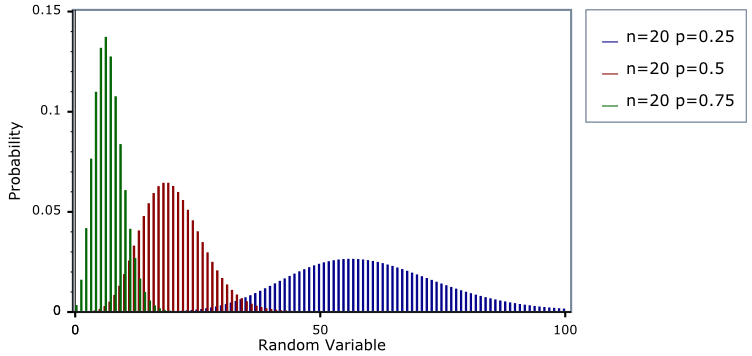
\includegraphics[width=.49\linewidth]{resources/negative_binomial_pdf_1.png}
  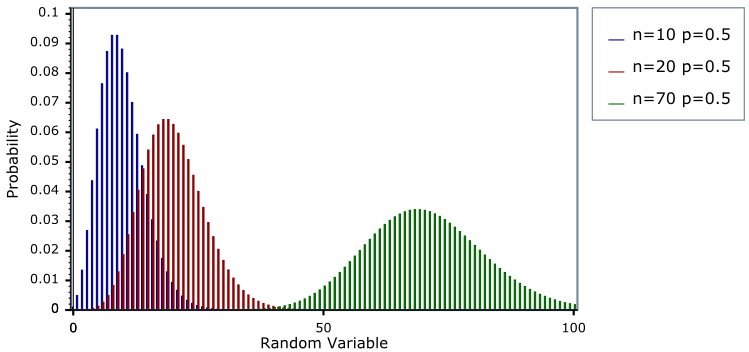
\includegraphics[width=.49\linewidth]{resources/negative_binomial_pdf_2.png}
\end{center}

\subsubsection*{The Expected Number of Successes}
The expected number of successes for $n$ Bernoulli trials with probability of success $p$ is
\[
  E[K] = np,
\]
where $K$ is the random variable denoting the number of successes in $n$ Bernoulli trials, and $E[K]$ is the expected number of successes.